% Template for Elsevier CRC journal article
% version 1.2 dated 09 May 2011

% This file (c) 2009-2011 Elsevier Ltd.  Modifications may be freely made,
% provided the edited file is saved under a different name

% This file contains modifications for Procedia Computer Science

% Changes since version 1.1
% - added "procedia" option compliant with ecrc.sty version 1.2a
%   (makes the layout approximately the same as the Word CRC template)
% - added example for generating copyright line in abstract

%-----------------------------------------------------------------------------------

%% This template uses the elsarticle.cls document class and the extension package ecrc.sty
%% For full documentation on usage of elsarticle.cls, consult the documentation "elsdoc.pdf"
%% Further resources available at http://www.elsevier.com/latex

%-----------------------------------------------------------------------------------

%%%%%%%%%%%%%%%%%%%%%%%%%%%%%%%%%%%%%%%%%%%%%%%%%%%%%%%%%%%%%%
%%%%%%%%%%%%%%%%%%%%%%%%%%%%%%%%%%%%%%%%%%%%%%%%%%%%%%%%%%%%%%
%%                                                          %%
%% Important note on usage                                  %%
%% -----------------------                                  %%
%% This file should normally be compiled with PDFLaTeX      %%
%% Using standard LaTeX should work but may produce clashes %%
%%                                                          %%
%%%%%%%%%%%%%%%%%%%%%%%%%%%%%%%%%%%%%%%%%%%%%%%%%%%%%%%%%%%%%%
%%%%%%%%%%%%%%%%%%%%%%%%%%%%%%%%%%%%%%%%%%%%%%%%%%%%%%%%%%%%%%

%% The '3p' and 'times' class options of elsarticle are used for Elsevier CRC
%% The 'procedia' option causes ecrc to approximate to the Word template
\documentclass[3p,times,procedia]{elsarticle}
\flushbottom

%% The `ecrc' package must be called to make the CRC functionality available
\usepackage{ecrc}
\usepackage[bookmarks=false]{hyperref}
    \hypersetup{colorlinks,
      linkcolor=blue,
      citecolor=blue,
      urlcolor=blue}
%\usepackage{amsmath}


%% The ecrc package defines commands needed for running heads and logos.
%% For running heads, you can set the journal name, the volume, the starting page and the authors

%% set the volume if you know. Otherwise `00'
\volume{00}

%% set the starting page if not 1
\firstpage{1}

%% Give the name of the journal
\journalname{Procedia Computer Science}

%% Give the author list to appear in the running head
%% Example \runauth{C.V. Radhakrishnan et al.}
\runauth{Brozeit et al.}

%% The choice of journal logo is determined by the \jid and \jnltitlelogo commands.
%% A user-supplied logo with the name <\jid>logo.pdf will be inserted if present.
%% e.g. if \jid{yspmi} the system will look for a file yspmilogo.pdf
%% Otherwise the content of \jnltitlelogo will be set between horizontal lines as a default logo

%% Give the abbreviation of the Journal.
\jid{procs}

%% Give a short journal name for the dummy logo (if needed)
%\jnltitlelogo{Computer Science}

%% Hereafter the template follows `elsarticle'.
%% For more details see the existing template files elsarticle-template-harv.tex and elsarticle-template-num.tex.

%% Elsevier CRC generally uses a numbered reference style
%% For this, the conventions of elsarticle-template-num.tex should be followed (included below)
%% If using BibTeX, use the style file elsarticle-num.bst

%% End of ecrc-specific commands
%%%%%%%%%%%%%%%%%%%%%%%%%%%%%%%%%%%%%%%%%%%%%%%%%%%%%%%%%%%%%%%%%%%%%%%%%%

%% The amssymb package provides various useful mathematical symbols

\usepackage{amssymb}
%% The amsthm package provides extended theorem environments
%% \usepackage{amsthm}

%% The lineno packages adds line numbers. Start line numbering with
%% \begin{linenumbers}, end it with \end{linenumbers}. Or switch it on
%% for the whole article with \linenumbers after \end{frontmatter}.
%% \usepackage{lineno}

%% natbib.sty is loaded by default. However, natbib options can be
%% provided with \biboptions{...} command. Following options are
%% valid:

%%   round  -  round parentheses are used (default)
%%   square -  square brackets are used   [option]
%%   curly  -  curly braces are used      {option}
%%   angle  -  angle brackets are used    <option>
%%   semicolon  -  multiple citations separated by semi-colon
%%   colon  - same as semicolon, an earlier confusion
%%   comma  -  separated by comma
%%   numbers-  selects numerical citations
%%   super  -  numerical citations as superscripts
%%   sort   -  sorts multiple citations according to order in ref. list
%%   sort&compress   -  like sort, but also compresses numerical citations
%%   compress - compresses without sorting
%%
%% \biboptions{authoryear}

% \biboptions{}

% if you have landscape tables
\usepackage[figuresright]{rotating}
%\usepackage{harvard}
% put your own definitions here:x
%   \newcommand{\cZ}{\cal{Z}}
%   \newtheorem{def}{Definition}[section]
%   ...

% add words to TeX's hyphenation exception list
%\hyphenation{author another created financial paper re-commend-ed Post-Script}

% declarations for front matter


\begin{document}
\begin{frontmatter}

%% Title, authors and addresses

%% use the tnoteref command within \title for footnotes;
%% use the tnotetext command for the associated footnote;
%% use the fnref command within \author or \address for footnotes;
%% use the fntext command for the associated footnote;
%% use the corref command within \author for corresponding author footnotes;
%% use the cortext command for the associated footnote;
%% use the ead command for the email address,
%% and the form \ead[url] for the home page:
%%
%% \title{Title\tnoteref{label1}}
%% \tnotetext[label1]{}
%% \author{Name\corref{cor1}\fnref{label2}}
%% \ead{email address}
%% \ead[url]{home page}
%% \fntext[label2]{}
%% \cortext[cor1]{}
%% \address{Address\fnref{label3}}
%% \fntext[label3]{}

\dochead{7th International Conference on Industry of the Future and Smart Manufacturing}%%%
%% Use \dochead if there is an article header, e.g. \dochead{Short communication}
%% \dochead can also be used to include a conference title, if directed by the editors
%% e.g. \dochead{17th International Conference on Dynamical Processes in Excited States of Solids}

\title{A Collection-based Digital Product Passport Suitable for Tracking Parts With No ID}

%% use optional labels to link authors explicitly to addresses:
%% \author[label1,label2]{<author name>}
%% \address[label1]{<address>}
%% \address[label2]{<address>}



\author[a]{Jonas Brozeit}
\author[a]{Abdullah Farrukh}
\author[a]{Peter Stein\corref{cor1}}
\author[a]{Christiane Plociennik}
\author[a]{Martin Ruskowski}
%\author[b]{System 180}

\address[a]{German Research Center for Artificial Intelligence (DFKI), Trippstadter Str. 122, 67663 Kaiserslautern, Germany}
% \address[b]{System 180 GmbH, Ernst-Augustin-Straße 3, 12489 Berlin, Germany}

\begin{abstract}
Digital Product Passports (DPPs) are great for collecting, tracking, and using product-related information across different stakeholders along the entire product lifecycle. Usually, a product is linked to its virtual counterpart (the DPP) by a machine-readable identifier (ID) such as a QR-code. An open question is how to seamlessly track products or parts of products that carry no ID on them. In this paper, we introduce a DPP concept based on the well-understood concept of a Collection. This approach assumes that each part belongs to a Collection at all times, which makes it trackable without an ID. An object can be removed from a Collection or added to another Collection. We explain our concept via a usecase from the System 180 Green-AI Hub pilot project.
\end{abstract}

\begin{keyword}
%% keywords here, in the form: keyword \sep keyword
Collection \sep Digital Product Passport \sep Circular Economy \sep Artificial Intelligence \sep Sustainability-oriented production \\


% more keywords: Digital Twins, Simulation, VR/AR Applications 

%% PACS codes here, in the form: \PACS code \sep code

%% MSC codes here, in the form: \MSC code \sep code
%% or \MSC[2008] code \sep code (2000 is the default)

\end{keyword}
\cortext[cor1]{Corresponding author.}
\end{frontmatter}

%\correspondingauthor[*]{Corresponding author. Tel.: +0-000-000-0000 ; fax: +0-000-000-0000.}
\email{jonas.brozeit@dfki.de}

%%
%% Start line numbering here if you want
%%
% \linenumbers

%% main text

%\enlargethispage{-7mm}



% Backup

% Introduction: State the objectives of the work and provide an adequate background, avoiding a detailed literature survey or a summary of the results. Focus on the original and outstanding contribution of your work compared to the state of the art.


% verschiedene Produkte sind eine Kollektion
% Eine Kollektion kann ein Möbelstück, aber auch ein Lager von Einzelteilen sein. Teile können einer Kollektion entnommen und einer anderen hinzugefügt werden. Da jedes Teil zu jeder Zeit einer Kollektion angehört, ist eine lückenlose Nachverfolgbarkeit jedes Teils gewährleiste
% 240711_Bewerbungsformular_Green-AI_Hub_Mittelstand_S180.pdf


% \begin{itemize}
%
%    \item Allgemeines Problem: Ressourcen wiederverwenden, verschwendung, bei komplexen Produkten, die verdefinierten Beziehungen 
%    \item Collection motivieren: Wir extrahieren DPP aus dem Bild, um wichtige Parameter darzustellen und zu analysieren. Digitales Lager ist Collection 
%    \item Wir erzeugen eine Collection zur strukturierten Verwaltung der Daten.
%    \item Outlook: - Teilmengen der Collection können mithilfe eines UI in andere Collections überführt werden (wichtig für Bestandsaufnahme und Collection-Management fürs Tracking).
%    \item  Verwendung von KG zur Analyse verdeckter Teile in der Collection.
%\end{itemize}

% /Backup

\section{Introduction}

The upcoming \emph{Ecodesign for Sustainable Products Regulation} (ESPR, COM/2022/142) will oblige many products, including furniture, to carry a \emph{Digital Product Passport} (DPP).  Manufacturers must therefore record each component’s composition, usage history, and end-of-life route.  Achieving that level of traceability in highly modular furniture is still an open challenge.

Modularized and extensible furniture systems are made up of smaller assemblies or singular parts with interconnections, which decrease the effort of reconfiguration and expansion while decreasing manufacturing complexity. System180 offers such a modular and extensible furniture system with various components which can be interconnected to fulfill a purpose, e.g. a shelf for an office or a workbench in a workshop. Besides using new parts to assemble a customer's furniture, the reuse of parts from furniture at the end of its lifecycle is a viable alternative. 

However, this requires careful examination and inventory of decommissioned furniture and its components. Due to the high variety of components, a manual process is not suitable for this task. The automation of the inventarisation task poses major challenges. To assess a component's lifecycle, it must be tracked across different lifecycle stages. Using unique identifiers, such as QR-codes or barcodes, is not feasible due to the large number of parts or lack of sufficient placement area on components.

Hence, this paper explores the use of state-of-the-art artificial intelligence (AI) methods, such as object detection and tracking, in combination with semantic technologies like the Asset Administration Shell (AAS), to automate the identification and classification of furniture components using image and video data.

To address the lack of physical identifiers, we apply the \textit{Collection Principle}, which structures digital product representations around dynamic groupings of parts. A collection may represent a physical product (e.g., a workbench), a stockpile, or an individual subassembly. Because each part always belongs to exactly one collection, the system ensures traceability without the need for permanent IDs. Collections can be interactively modified via a user interface, allowing users to transfer subsets into new or existing collections—supporting processes such as inventory audits, reassembly, or reuse planning.

Additionally, we store all detected relationships and metadata in a Neo4j knowledge graph. This enables advanced queries and inference, including reasoning over components that are not directly visible in an image but may be inferred based on their likely inclusion within a known configuration or context.

We assess the concept using two complementary demonstrators: (1) a web-based application that allows users to upload or capture component images, and (2) a physical demonstrator using embedded hardware and cameras to capture and classify components on-site. With this work, we aim to contribute to key goals of the circular economy and Industry 4.0 by making modular furniture more reusable, identifiable, and semantically linked across its lifecycle.

%%% Backup 

% \subsection{Related Work}

% Training
% Training AI models to detect and track components of a furniture piece using images and videos, training data is needed. Besides using real data, which is annotated by domain experts manually using labeling tools (\cite{Labelstudio}, \cite{dwyer2024roboflow}), synthetic data is utilized. As the authors of \cite{ICPSPaper} showed, using synthetic data, generated using a graphic API \cite{schieber_indoor_2024}, can be a viable option to train or pretrain an AI detection model. The synthetic data includes RGB images and 2D bounding box annotation for various furniture components and is generated using Isaac-Sim \cite{Isaac-Sim}. 

%%%%%

\section{Related Work}

Training AI models to detect and track components of modular furniture requires suitable datasets. Besides real-world data—typically annotated manually by domain experts using labeling tools such as Label Studio~\cite{Labelstudio} or Roboflow~\cite{dwyer2024roboflow}—synthetic data can be used to augment or bootstrap model training. Simulation platforms such as Isaac-Sim~\cite{Isaac-Sim} can generate diverse and precisely annotated RGB images, offering scalable training input for object detection models.

Recent literature has demonstrated the effectiveness of deep learning for identifying modular components in structured assemblies. Ramesh et al.~\cite{ramesh2024investigation} compared multiple models for detecting fasteners in rail assemblies, showing that YOLOv5 significantly outperforms Mask R-CNN with over 99\,\% mAP, making it suitable for real-time component recognition in industrial settings.

Siao et al.~\cite{siao2024furniture} present a domain-specific application in system furniture manufacturing, where CNN-based automated optical inspection (AOI) is used to verify completeness of furniture kits before packaging. This mirrors our goal of ensuring component integrity in configurable modular assemblies.

Tian et al.~\cite{tian2025inspection} build on YOLOv11 with enhancements such as RepViT and multi-scale feature fusion to detect peg-and-hole components under occlusion and angle variation—challenges common in reused or cluttered configurations. This supports our use of advanced YOLOv11 variants for robust detection.

For tracking and identifying unlabeled components, Eisenbach et al.~\cite{eisenbach2024} propose a class-agnostic detector combined with object re-identification. This enables detection of unseen parts without fine-tuning—critical in reuse contexts with unknown or unlabeled parts, and conceptually aligned with our ID-free Collection approach.

In summary, prior work confirms the feasibility of AI-based modular component detection, both in general assembly and furniture-specific domains. However, none of these approaches integrate detection results into a dynamic, graph-based lifecycle model. Our work fills this gap by linking vision-based recognition with a Digital Product Passport system using semantic graph representations for tracking parts without physical identifiers.



% \begin{itemize}
%     \item AbFa: ICPS Paper, Synthetische Daten
%     \item JoBr: CircThread, Objekterkennung verknüpft mit DPP in der Kreislaufwirtschaft and Wiederverwendung, 
%     \item PeSt: Objekterkennung und Zustandserkennung von verschiedenen (komplexen) Komponenten /Möbel
%     \item ChPl: ReCirce - zentraler DPP?
% \end{itemize}

\section{Methodology}

\subsection{Requirements}

\section{Proof of Concept}

\section{Discussion}

\section{Conclusion and Outlook}

\subsection{Collection}
%\begin{itemize}
%    \item tracking von teilen ohne ID - Auftrags-ID 
%\end{itemize}\textbf{}

The instantiated DPP of a product can, much like the real counterpart, be stored in a storage. This digital storage, realized using databases, allows creating relationships between individual DPPs. Using these relationships, the composition of a real product can be modelled in the digital storage by creating collections. A collection is a summary of relationships of different DPPs, which can be used to track the components of a product during their lifecycles. Using collections, components of a product can be transferred to a collection of another product as a subset using the DPP, hence enabling the tracking of products without unique identification. If components of a decommissioned product at the end of the lifecycle are reused to manufacture a new product, the collection of the new product is extended by the subset of the collection of the decommissioned product.


\section{Material and methods}
% Material and methods: Provide sufficient details to allow the work to be reproduced by an independent researcher. Methods that are already published should be summarized, and indicated by a reference. If quoting directly from a previously published method, use quotation marks and also cite the source. Any modifications to existing methods should also be described.

\subsection{Requirements}

The requirements for the AI-based object recognition system were derived from an analysis of the furniture components. The identified requirements take into account the specific technical and operational challenges associated with implementing computer vision technologies for sustainable inventory management in modular furniture systems. These requirements arose from the need to establish efficient material flow tracking while supporting circular economy business models through advanced artificial intelligence applications.\\

funktionale Req\\

nicht funktionale Req\\

\begin{itemize}
    \item KI - Objekterkennung
    \item Ressourceneffizienz
    \item Komplexe Kombination der Bauteile  und Produktvielfalt
    \item Nutzbar durch jeden Bild and videodaten als eingang --\> Unterschiedliche Perspektiven, Winkel, Kameraauflösung, etc. Messen 
    \item nachtrainierbar
    \item moderne Softwaremethoden CI/CD
    \item webanwendung
    \item confidence von xx % 
    \item Angereicherter DPP durch Datenbank
    \item Open source 
\end{itemize}


\subsection{Methodology}

% TODO: Exact size of each dataset (real photos vs. synthetic images). 
% TODO: YOLOv11 training details – epochs, batch size, LR schedule, augmentation.
% TODO: Hardware specs (GPU, Jetson Orin settings, inference engine used).
% TODO: FastAPI + Neo4j deployment architecture (container image, queue, REST endpoints).


\begin{figure}
    \centering
    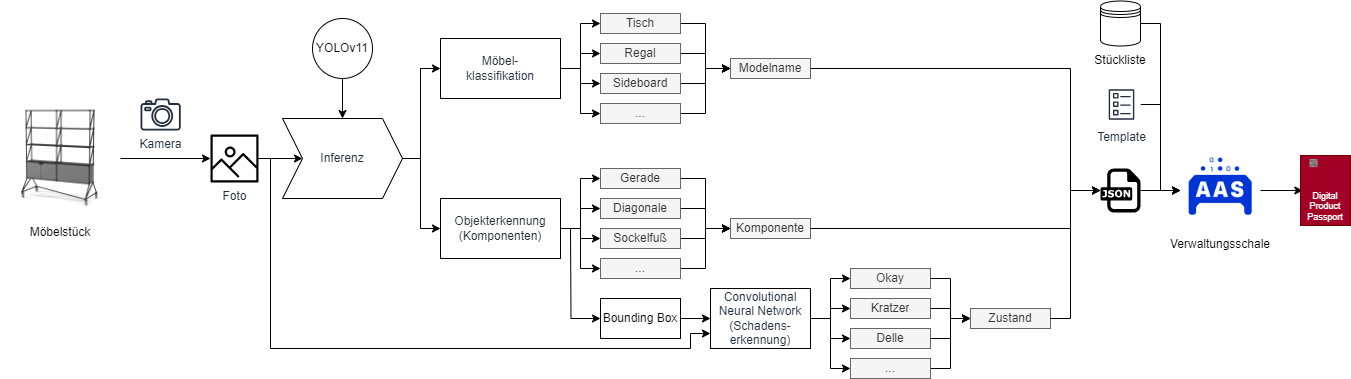
\includegraphics[width=1\linewidth]{images/concept.png}
    \caption{Concept}
    \label{fig:concept}
\end{figure}
% https://dfkide.sharepoint.com/:p:/s/Team_GAIHSystem180-GemeinsamesTeams/EZU6vO42ZEhGk-IK9XiSic0Br72q1NsNtXn235TGDAtPUQ?e=zqcrCB

The DPP of a product requires various data points. Many of the data points can be obtained from pre-existing documents, databases etc., but others require an assessment by inspecting the product, e.g. part condition. This can be done manually, which is labour-intensive and time-consuming or automated using AI tools. In our study, two use-cases were analyzed:
\begin{itemize}
    \item Generating a bill of material as a collection using image and video data  
    \item Precommissioning and condition assessment of furniture components image and video data
\end{itemize}

...
Training data is required to enable the detection, tracking and assessment of the condition of the parts using AI models.  

Konzept erklären - wie wollen wir es umsetzen? (Bild erklären)
Eingang: bild and videodaten als eingang\\
Überleitung: für training brauchen wir daten und die real und synthetisch 

\subsection{training (AbFa) - umnenenn }
Training, Label von Fotos und synthetischen Daten\\
Zustandserkennung (pytorch - PeSt) \\
Labeling: roboflow,  (JoBr)\\
ultralytrics YOLO welche Modelle v8,v10,v11
daten selbst trainieren 



\subsection{information extraction and visualisierung }
\begin{itemize}
    \item ai based - feature erkennung (farbe, länge) + decor anpassung erweiterung \\ 
    Zustandserkennung, Qualitätserkennung \\
    Messen (Aruco Marker und Referenzwerten)
    \item topologie - Ansätze von VLM (Hooman)
\end{itemize}

\subsection{überführung in DPP (Neo4J) }

\begin{itemize}
      \item Webanwendung und Produktionsdemonstrator.
      \item Graph based DPP (Neo4j): Application Ressourceneffizient und Transportemissionen kalkulation
\end{itemize}


\section{Results}

% TODO:  Quantitative model metrics (mAP@0.5, precision-recall, IoU for nubs detection).
% TODO: Inference speed (fps) on Jetson Orin & on server-class GPU.
% TODO: End-to-end latency web-upload → Neo4j write.
% TODO: Storage footprint per item / graph query latency (optional).

% Results: Results should be clear and concise. 

\subsection{Proof of Concept - (JoBr, PeSt, AbFa)}
\begin{itemize}
    \item Implementation in Demonstrator (WebUI und SUPSEKT - Demonstrator
    \item Open Source
\end{itemize}

\begin{figure}
    \centering
    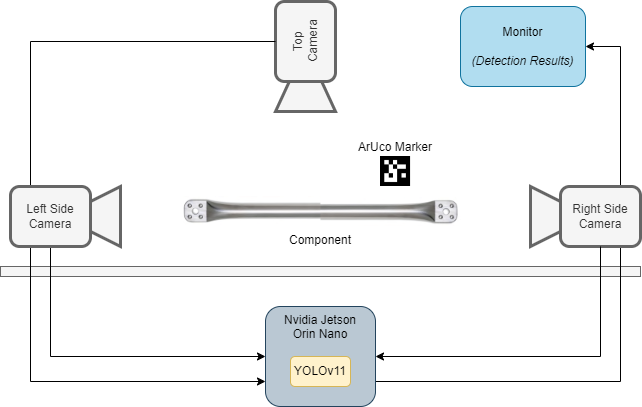
\includegraphics[width=.6\linewidth]{images/demonstrator.png}
    \caption{Demonstrator}
    \label{fig:demonstrator}
\end{figure}

- Hardware requirements 4 Objekte
- funktioniert auf Rechenschwachen PC/Handy

\section{Discussion -  (vor Orttermin, alle zusammen schreiben)}
% Discussion: This should explore the significance of the results of the work, not repeat them. A combined Results and Discussion section is often appropriate. Avoid extensive citations and discussion of published literature.

\begin{itemize}
    \item Aktuelle Technologien ermöglichen das tracken von Objekten ohne eindeutige IDs
    \item KI-methoden ermöglichen die Informationsextrahierung für DPP als Bild und Video daten --\> EU Call  ai based Services to fill DPP
    \item Syntheische Daten führen zu schnellen Erfolgen, anreichern von Trainingsdaten/ erweiterbarkeit / ai-operationalization  
    \item VLM geeignet um aus Bilddaten zu inferieren (aus zwei kompontenen "beziehung" finden) und fehlende Objekte zu finden 
    \item Standards Einheitliches Vokabular - Interoperability, Ontologien Taxonomien, OPD paper, VWS hinzufügen
\end{itemize}



\section{Conclusion and Outlook}
% The main conclusions of the study may be presented in a short Conclusions section, which may stand alone or form a subsection of a Discussion or Results and Discussion section.
unsere arbeit zeigt, dass das Konzept funktioniert, Skalierbar, schwachstellen in den bereichen weitere papieren ausgeführt werden muss. 
Disassembly von teilen etc 



\section{Acknowledgements}

\bibliography{references}
\bibliographystyle{elsarticle-harv}

\end{document}

